% -*- TeX:RNW:UK -*-
\documentclass[10pt]{beamer}
\usetheme{metropolis}
%\useinnertheme{rectangles}'
\setbeamercovered{%
still covered={\opaqueness<1->{15}},
again covered={\opaqueness<1->{40}}}

\hypersetup{colorlinks,linkcolor=black,urlcolor=brown,citecolor=brown}

\usepackage{amsmath,amssymb,amsthm}
\usepackage{unicode-math}

% We set the Lucida OTF fonts as default
\usepackage{fontspec}
\setmainfont{Lucida Bright OT}
\setsansfont{Lucida Sans OT}
\setmonofont{Lucida Console DK}[Scale=MatchLowercase]

\newfontfamily\typiconsfont{Typicons}[Scale=0.9]
\newcommand\typicons[1]{{\typiconsfont\symbol{#1}}}
\newcommand\Attention{\colorbox{yellow}{\textcolor{black}{\typicons{"E136}}}\xspace}
\newcommand\Advanced{\colorbox{black}{\textcolor{white}{\typicons{"E04E}}}\xspace}

\newfontfamily\webglyphsfont{WebHostingHub-Glyphs}[Scale=0.7]
\newcommand\webglyphs[1]{{\webglyphsfont\symbol{#1}}}
\newcommand\Discussion{\colorbox{white}{\textcolor{black}{\webglyphs{"F134}}}\xspace}
\newcommand\DExamples{\colorbox{black}{\textcolor{white}{\webglyphs{"F134} examples?}}}
\newcommand\Reading{\colorbox{black}{\textcolor{white}{\webglyphs{"F0C1}}}\xspace}

\newfontfamily\meteoconsfont{Meteocons}
\newcommand\meteocons[1]{{\meteoconsfont\symbol{#1}}}
\newcommand\meteosun{\meteocons{"0042}}
\newcommand\meteosuncloud{\meteocons{"0048}}
\newcommand\meteorain{\meteocons{"0052}}
\newcommand\meteosolidsun{\meteocons{"0031}}

\newfontfamily\KRfarmfont{KR Back On The Farm}
\newcommand\KRfarm[1]{{\KRfarmfont\symbol{#1}}}
\newcommand\farmplant{\KRfarm{"0049}}

\usepackage{polyglossia}
\setdefaultlanguage[variant = british, ordinalmonthday = false]{english}

\usepackage[style=authoryear-comp,firstinits,sortcites,maxcitenames=2,%
    mincitenames=1,maxbibnames=10,minbibnames=10,uniquename=mininit,%
    uniquelist=minyear,sortfirstinits=true]{biblatex}
\addbibresource{../references/ecophys.bib}
%\renewcommand{\bibfont}{\small}

\usepackage{abbrev}
\DeclareGraphicsExtensions{.png,.jpg,.jpeg,.eps,.pdf}


\title{Physiological Plant Ecology\\
       Lecture 13: Water Relations}
\author{Pedro J. Aphalo}
\date{September--October 2013}

\begin{document}


\title{PBIO-141\\Sensory and Physiological Ecology of  Plants}
\subtitle{14: Energy balance}
\author{Pedro J. Aphalo}
\date{January-February 2018}
\institute[Univ.\ of Helsinki]{M.Sc.\ in Plant Biology, University of Helsinki\\[2ex] \url{http://blogs.helsinki.fi/aphalo/}}


  \begin{frame}
    \maketitle
  \end{frame}

  \begin{frame}[c]
    \begin{center}
      \begin{small}
        \copyright 2006-2018 by Pedro J. Aphalo\\
       University of Helsinki, Finland.\\
        \textcolor{blue}{\url{http://blogs.helsinki.fi/aphalo/}}\\[2ex]
      \end{small}

      \begin{footnotesize}
        Sensory and Physiological Ecology of  Plants: `14: Energy balance' by Pedro J. Aphalo is licensed under a Creative Commons Attribution-ShareAlike 4.0 International License.

        Illustrations and text quoted from copyrighted sources is excluded from this license and their use should respect the original licenses.\\[2ex]
      \end{footnotesize}

      \centering\centering
\includegraphics[width=6em]{../figures/copyright/by-sa}
    \end{center}
  \end{frame}

  \begin{frame}
    \frametitle{Outline}
    \tableofcontents
  \end{frame}

\section{Energy balance}

\begin{frame}{Radiation balance of a leaf}
    \begin{itemize}
        \item Every object emits radiation according to its
        temperature.
        \item Every object absorbs radiation from its
        environment.
        \item Absorptivity and emissivity ($\varepsilon$) indicate the fraction of
        irradiance absorbed, and the fraction of the ideal emission
        emitted.
        \item Absorptivity and emissivity depend on the wavelength,
        but at a given wavelength are numerically equal.
        \item A \emph{black body}, a theoretical concept, absorbs
        all radiation incident on it (absorptivity = 1, $\varepsilon$ = 1).
    \end{itemize}
\end{frame}

\begin{frame}{Emitted radiation}
    \begin{itemize}
        \item The radiation emitted by a body depends on its
        temperature, and its emissivity.%
        \item A cold object emits less radiation and at longer
        wavelengths than a body at higher temperatures.%
        \item The sun emits radiation as a black body at 5800 K
        (degrees Kelvin). This is called by meteorologists shortwave radiation.%
        \item A leaf will emit according to its temperature, at
        much longer wavelengths than the sun. This is called by
        meteorologists longwave radiation.
    \end{itemize}
\end{frame}

\begin{frame}{Emitted radiation}
    \begin{itemize}
        \item At ambient temperatures it is normally assumed for
        plants, animals and water that they are perfect emitters
        ($\varepsilon=1$).
        \item $\boldmath{F} = \varepsilon \sigma T_s^4$, where $F$
        is the flux of energy emitted, $\varepsilon$ the emissivity, $\sigma$
        is Stefan Boltzmann's constant, and $T_s$ is the absolute
        temperature of the surface of the emitting object.
        \item At around 280 K most of the energy is in the
        waveband 5--25 $\mu$m.
    \end{itemize}
\end{frame}

\begin{frame}{Absorptance of a leaf}
    \begin{itemize}
        \item Of the shortwave radiation, visible radiation is
        strongly absorbed and near-IR poorly absorbed,
        \item Longwave radiation is strongly absorbed.
    \end{itemize}
\end{frame}

\begin{frame}{Spectrum}
    \centering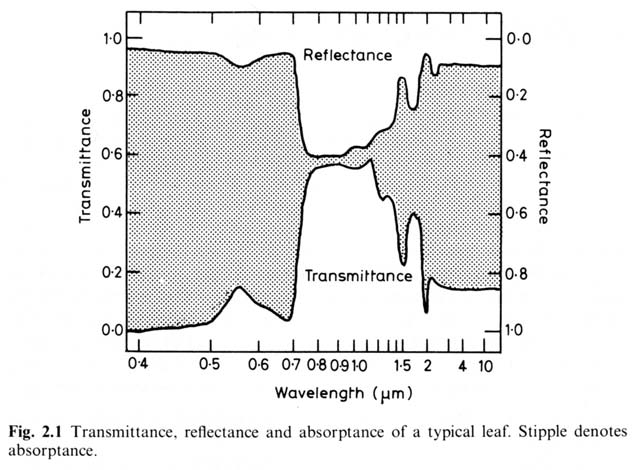
\includegraphics[height=0.7\textheight]{figures/Grace2.1LeafSpectrum.eps}\\
    {\small \autocite[from][]{Grace1983}.}
\end{frame}

\begin{frame}{Radiation balance of a leaf}
    \centering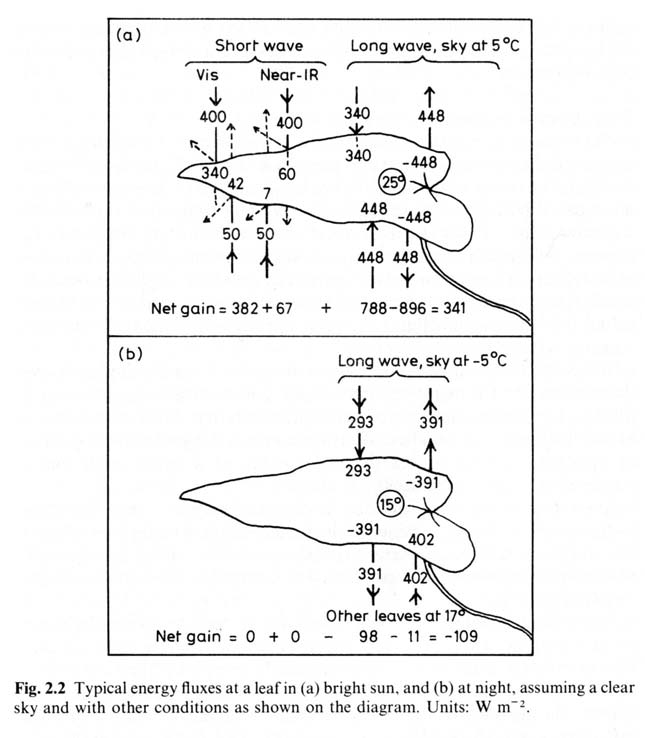
\includegraphics[height=0.75\textheight]{figures/Grace2.2EnergyLeaf.eps}\\
    {\footnotesize the equation in panel (b) of the figure should read\\
    Net gain $=0+0-98+11=-87$}\\
     {\small \autocite[from][]{Grace1983}.}
\end{frame}

\begin{frame}{Radiation profile}
    \centering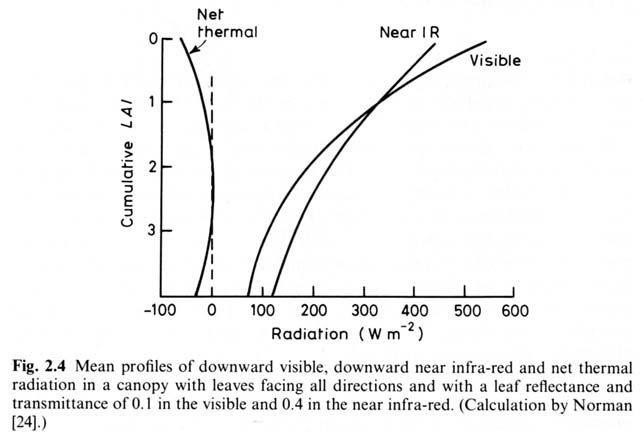
\includegraphics[width=0.95\textwidth]{figures/Grace2.4RadiationProfileCanopy.eps}\\
    {\small \autocite[from][]{Grace1983}.}
\end{frame}

\begin{frame}{Energy balance}
    Heat gains by radiation = heat losses:
    $$\boldmath R = \lambda E + C + S + G + P,$$%
    \begin{small}
    where $\boldmath R$ is the net heat gain through radiative
    exchanges, $\lambda$ is the heat of vaporization, $\boldmath E$
    is the evaporation and/or transpiration rate, $\boldmath C$ is
    the heat lost by convection, $\boldmath S$ is the heat that goes
    into storage in the leaf (change in temperature), $\boldmath G$
    is the conduction of heat down the petiole, and $\boldmath P$ is
    the energy trapped in chemical bonds through photosynthesis.
    \begin{itemize}
        \item All terms in energy flux units (W m$^{-2}$).
        \item $\boldmath G$ and $\boldmath P$ are very small in
        most situations, and $\boldmath S$ can be ignored if we assume that
        temperature of the leaf is in equilibrium.
    \end{itemize}
    \end{small}
\end{frame}

\begin{frame}{Leaf temperature}
    \centering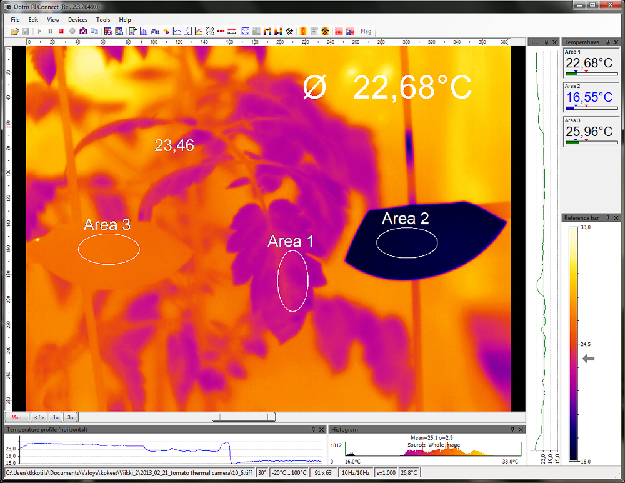
\includegraphics[width=0.9\textwidth]{figures/Tomato_IR_Valoya-.eps}
\end{frame}

\section{Adaptation and acclimation}

\begin{frame}{High reflectance as an adaptation}
    \begin{itemize}
        \item Some plants have leaves that reflect more light than
        what is usual.
        \item Leaves are covered with hairs (pubescence) or waxes.
        \item[$\circ$] (In some other species hairs reflect little light
        but increase the thickness of the boundary layer.)
        \item These are mostly desert plants.
        \item Increasing visible light reflectance contributes to
        lower leaf temperatures in full sunlight.
        \item In some species there is also acclimation: hairiness
        depends on the season when leaves are formed.
    \end{itemize}
\end{frame}

\begin{frame}{Encelia farinosa}
    \centering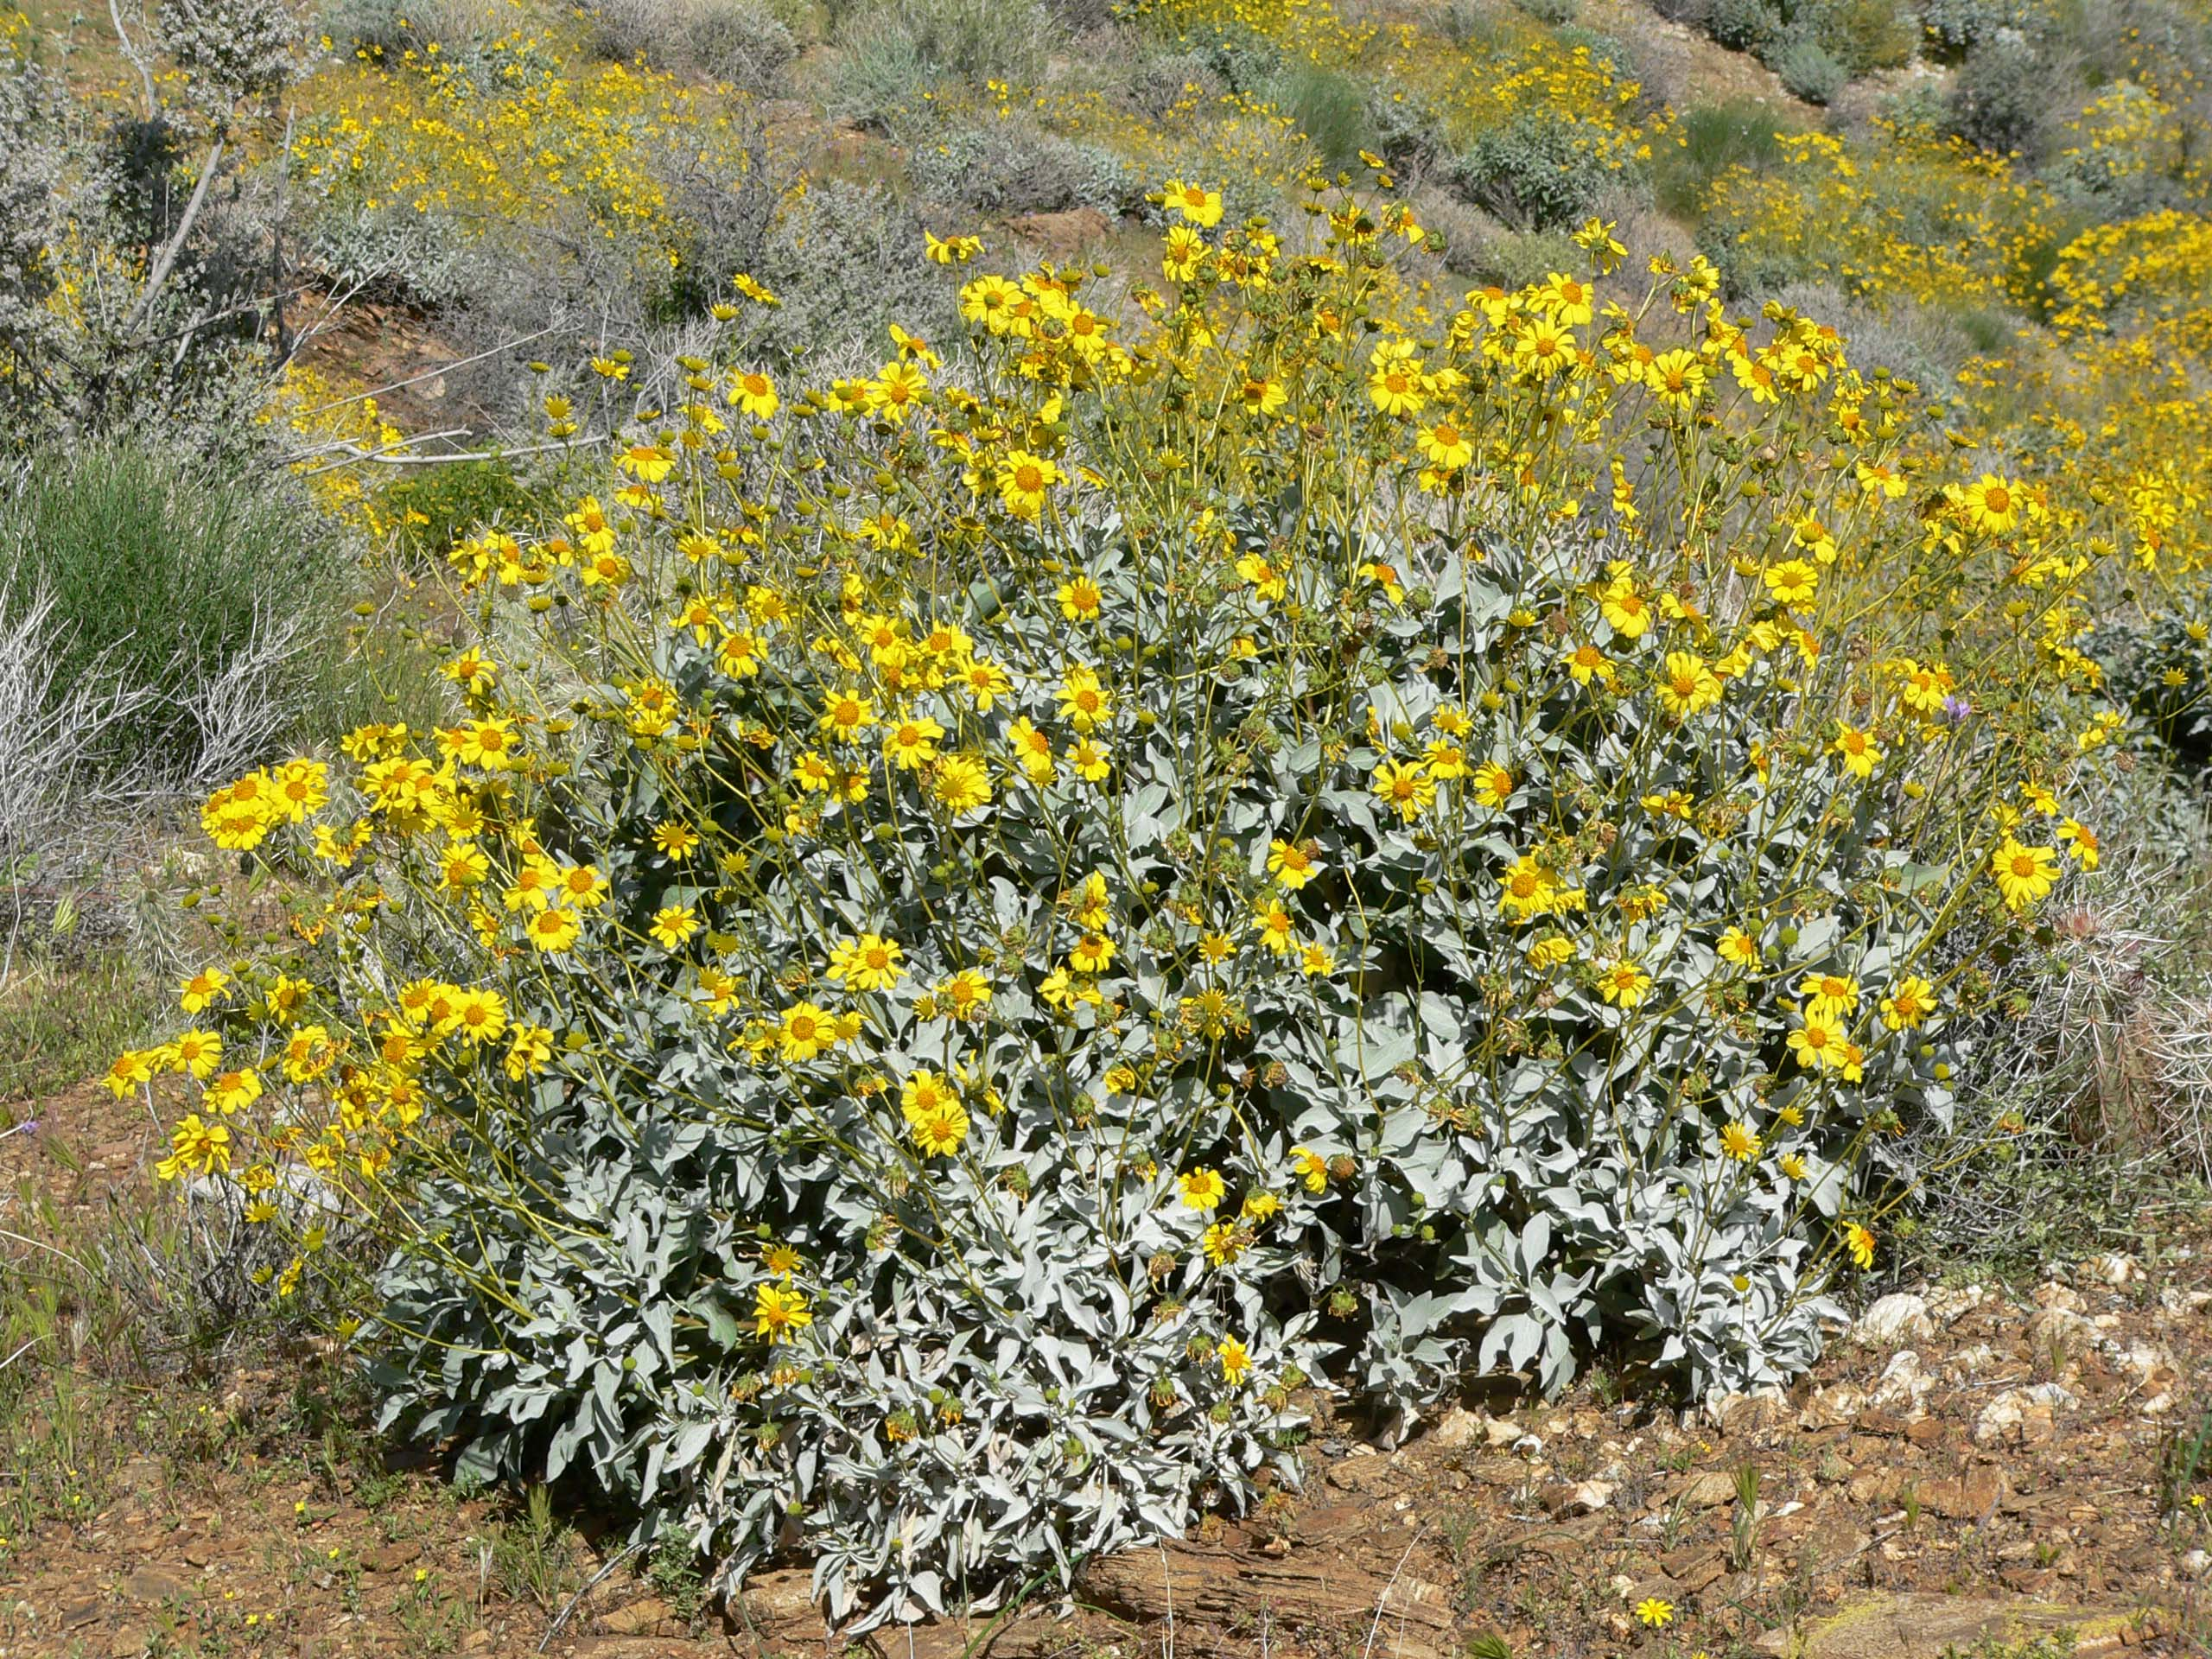
\includegraphics[height=0.7\textheight]{figures/Encelia_farinosa.eps}\\
    {\tiny FDL (from \url{http://en.wikipedia.org/wiki/Image:Encelia_farinosa_form.jpg}.}
\end{frame}

\begin{frame}{Pubescence and temperature}
    \centering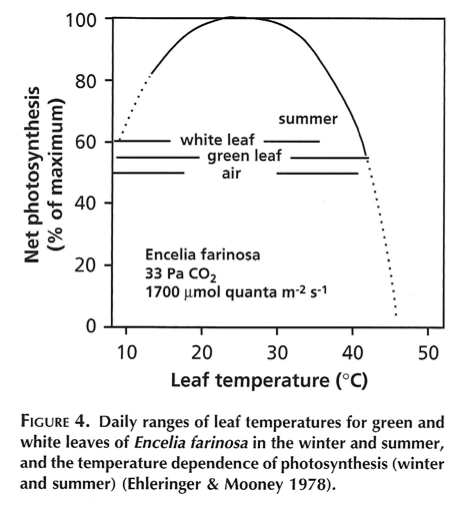
\includegraphics[height=0.7\textheight]{figures/Lambers4Encelia.eps}\\
    {\small \autocite[from][]{LambersEtAl1998}.}
\end{frame}

\begin{frame}{Leaf size}
    \centering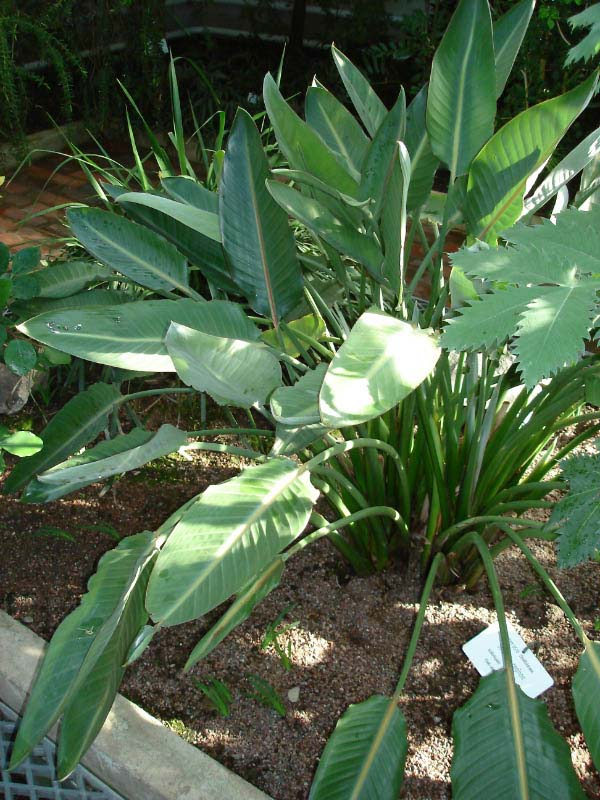
\includegraphics[width=0.45\textwidth]{figures/Sterlitzia.eps}%
    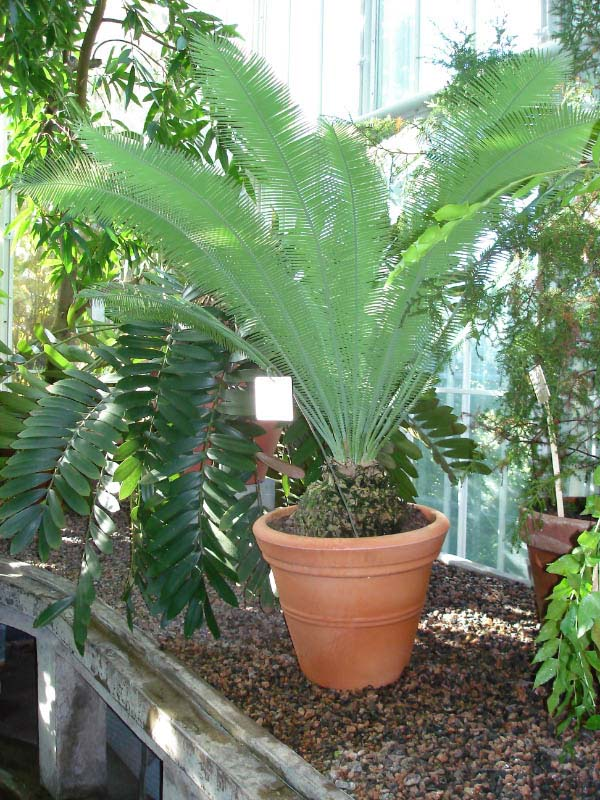
\includegraphics[width=0.45\textwidth]{figures/Palm.eps}\\
\end{frame}

\begin{frame}{Leaf size}
    \centering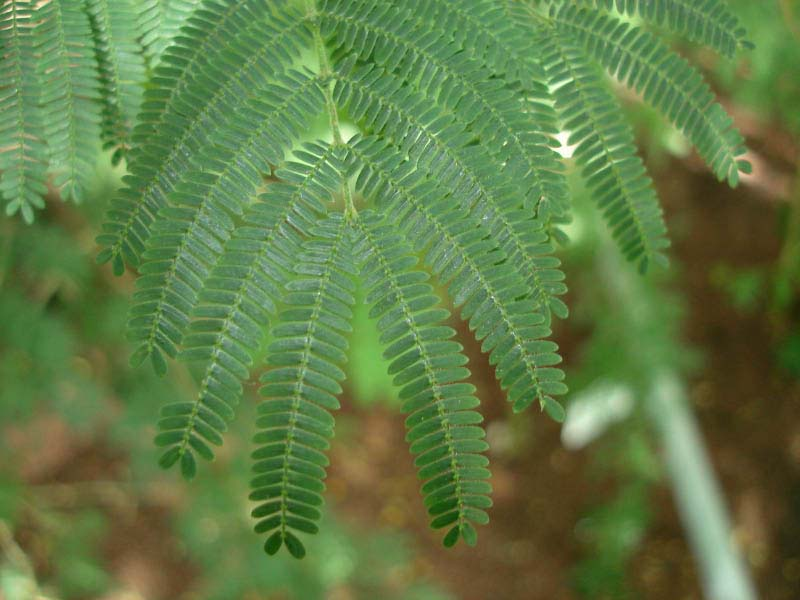
\includegraphics[width=0.47\textwidth]{figures/Mimosoidea.eps}%
    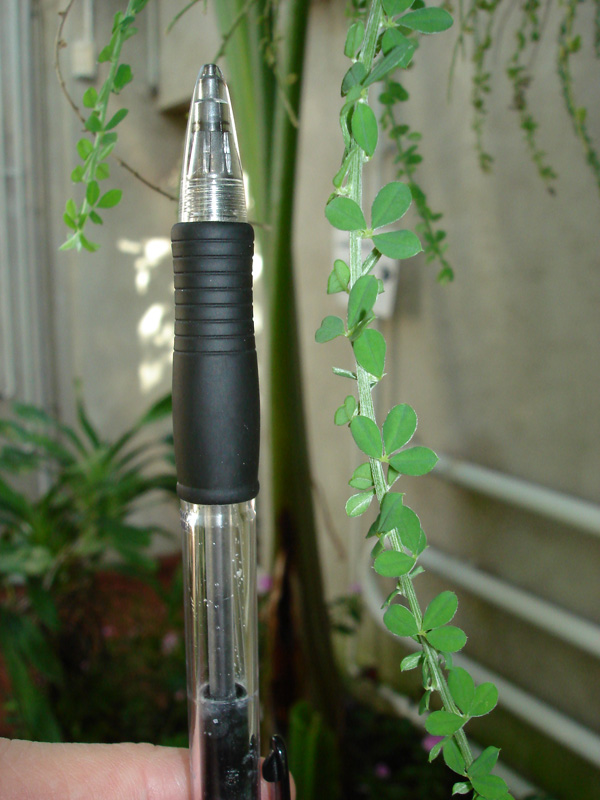
\includegraphics[width=0.47\textwidth]{figures/SmallLeaves.eps}
\end{frame}

\begin{frame}{Leaf size}
    \begin{itemize}
        \item Different species have very different sizes of
        leaves.
        \item Some have composite leaves with leaflets of
        different sizes.
        \item Leaf margins vary (entire, with teeth, etc.)
        \item Size and shape affect the aerodynamic properties of
        leaves, and so the thickness of the boundary layer.
        \item The boundary layer in turn affects gas exchange and
        the energy balance ($E$ and $C$ change).
        \item This is reflected in the temperature of the leaf.
    \end{itemize}
\end{frame}

\begin{frame}{Coupling}
    \begin{itemize}
        \item The temperature of small leaves is tightly coupled
        to that of the air. (Differences in temperature are small.)
        \item The temperature of big leaves is not tightly
        coupled to that of the air. (Differences in temperature can be large.)
        \item Small leaves are common in arid regions.
        \item Large leaves are common in the humid tropics,
        specially in the understorey of the forest.
        \item Some leaves are large, like those of some palm
        trees, but because their blade in broken up into small
        pieces function as much smaller leaves.
    \end{itemize}
\end{frame}

\begin{frame}{}
    \centering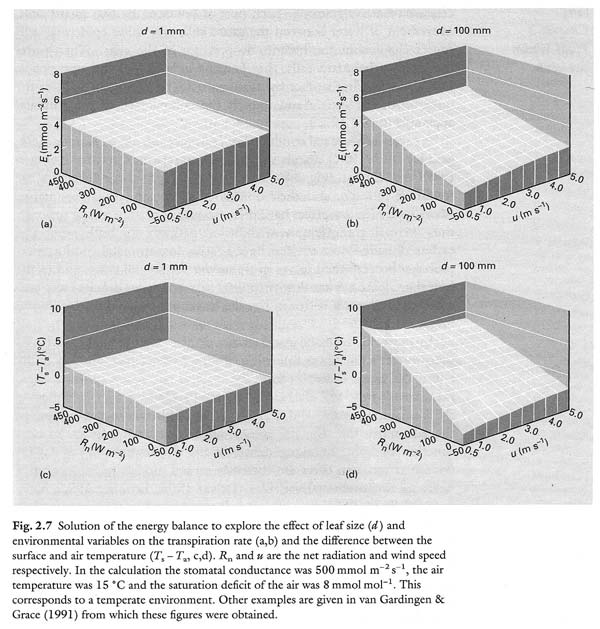
\includegraphics[height=0.95\textheight]{figures/Crawley2.7LeafSizeEnergyBalance.eps}\\
    {\small \autocite[from][]{Crawley1997}.}
\end{frame}

\begin{frame}{Evaporative cooling}
    \begin{itemize}
        \item When a leaf loses water through transpiration,
        water evaporates in walls of mesophyll cells.
        \item Evaporation uses energy, and this cools the leaf.
        (Conversely condensation during dew formation warms slightly
        the leaf.)
        \item In hot climates, if transpiration would stop completely
        at midday temperature of the leaf would rise over the lethal
        threshold.
    \end{itemize}
\end{frame}

\begin{frame}{Evaporative cooling}
    \centering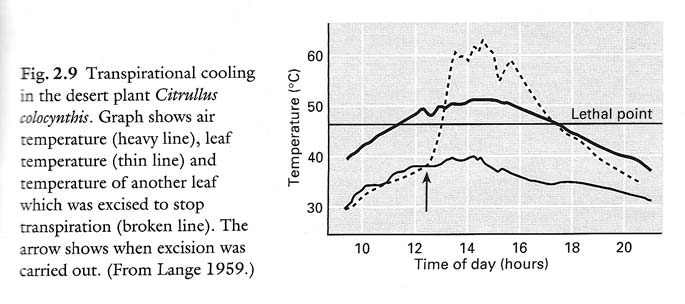
\includegraphics[width=\textwidth]{figures/Crawley2.9LeafLethalTemperature.eps}\\
    {\small \autocite[from][]{Crawley1997}.}
\end{frame}

\begin{frame}{Leaf display and heliotropism}
    \begin{itemize}
        \item Leaves of many plants move, but so slowly that we
        usually do not notice it.
        \item This affects radiation (shortwave and
        longwave) interception.
        \item Which in turn alters leaf temperature, and
        photosynthetic rate.
        \item Even when they do not move, the position of leaves
        affects their radiation balance.
    \end{itemize}
\end{frame}

\begin{frame}{Leaf display and heliotropism}
    \begin{description}
        \item[Diaheliotropism] Leaves track the movement of the
        sun, keeping the leaf blade perpendicular to the sunlight beam.
        \item[Paraheliotropism] Leaves track the movement of the
        sun, keeping the leaf blade parallel to the sunlight beam.
        \item[Nictinasty] Leaves move during the night, normally
        to a vertical position. Sometimes elaborate folding of
        leaflets.
    \end{description}
\end{frame}

\begin{frame}{Nictinasty}
    \centering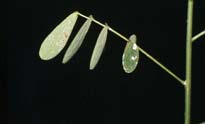
\includegraphics[width=0.33\textwidth]{figures/Cassia_1.eps}%
    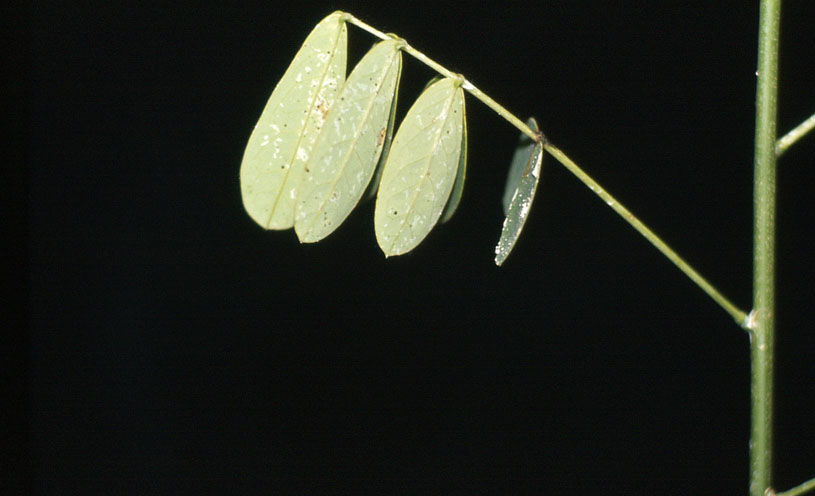
\includegraphics[width=0.33\textwidth]{figures/Cassia_2.eps}%
    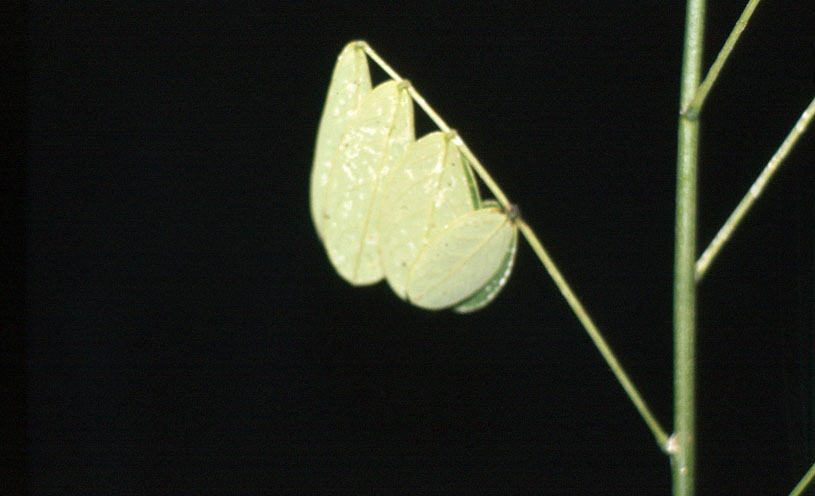
\includegraphics[width=0.33\textwidth]{figures/Cassia_3.eps}\\
    \textit{Cassia bicapsularis}.
\end{frame}

\begin{frame}{Leaf display and heliotropism}
    \centering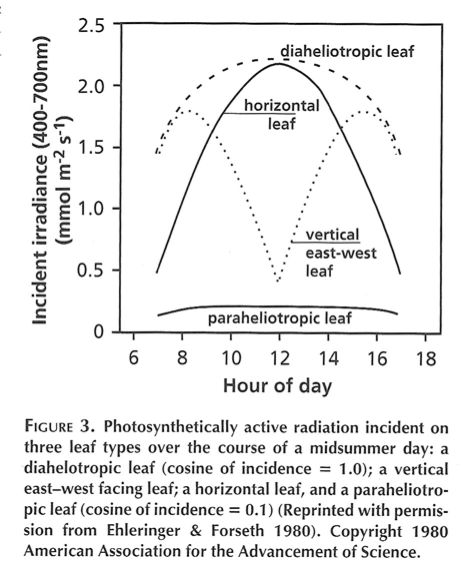
\includegraphics[height=0.7\textheight]{figures/Lambers3HeliotropicIrradiance.eps}\\
    {\small \autocite[from][]{LambersEtAl1998}.}
\end{frame}

\begin{frame}{Leaf rolling}
    \fbox{\includegraphics[height=0.7\textheight]{figures/Maize_0_small.eps}}%
    \fbox{\includegraphics[height=0.7\textheight]{figures/Maize_2_small.eps}}\\
    Maize, left: well watered, right: not watered.
\end{frame}

\section{Boundary layer and canopies}

\begin{frame}{Boundary layer of a leaf}
    \centering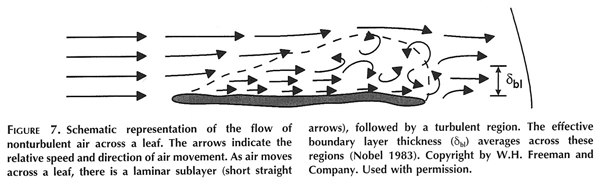
\includegraphics[width=\textwidth]{figures/Lambers7BoundaryLayer.eps}\\
    {\small \autocite[from][]{LambersEtAl1998}.}
\end{frame}

\begin{frame}{Wind speed profiles}
    \centering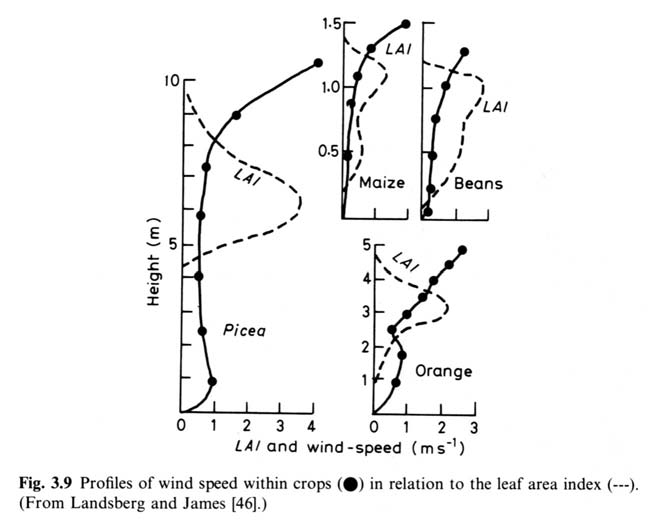
\includegraphics[height=0.70\textheight]{figures/Grace3.9WindProfile.eps}\\
    {\small \autocite[from][]{Grace1983}.}
\end{frame}

\begin{frame}{Water and temperature profiles}
    \centering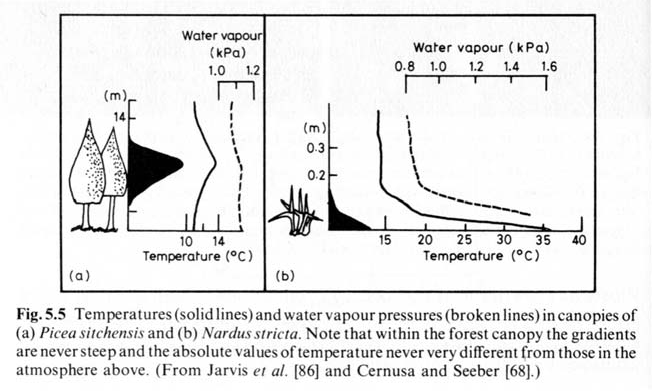
\includegraphics[width=\textwidth]{figures/Grace5.5WaterTempProfileCanopies.eps}\\
    {\small \autocite[from][]{Grace1983}.}
\end{frame}

\section*{References}

  \begin{frame}[t,allowframebreaks]
    \frametitle{References}
    \printbibliography
  \end{frame}

\end{document}

\section{References}
\begin{frame}{References}
\bibliographystyle{abbrvnat}
\nobibliography{ecophys_course_lectures}
\begin{footnotesize}
% \hangbibentry{AphSan1986}

% \hangbibentry{Aphalo1991}

% \hangbibentry{AphaloEtAl1991}

 \hangbibentry{Crawley1997}

% \hangbibentry{EhlOsm1991}

% \hangbibentry{EvansEtAl1988}

% \hangbibentry{Givnish1988}

 \hangbibentry{Grace1983}

% \hangbibentry{Heldt1997}

% \hangbibentry{KozlowskiEtAl1991}

 \hangbibentry{LambersEtAl1998}

% \hangbibentry{Larcher2003}

% \hangbibentry{Lawlor1987}

% \hangbibentry{Lichtenthaler1985}

% \hangbibentry{OsmCho1988}

\hangbibentry{TaiZei2006}

% \hangbibentry{WilFri1996}

\end{footnotesize}
\end{frame}


